\newcommand{\psd}[1]{{\small\sffamily{\color{blue!60}#1}}}

To showcase the usage of linear elasticity with more than one Dirichlet
condition, we shall discuss here an example of a 2D bar which bends
under its own load. The same problem from previous tutorials 1 and 2 is
used here, a bar 5 m in length and 1 m in width, and is supposed to be
made up of a material with density \(\rho=8\times 10^3\), Youngs modulus
\(E=200\times 10^9\), and Poissons ratio \(\nu=0.3\). Contrary to
tutorials 1 and 2, now both ends of the bar are clamped (mathematically,
two Dirichlet conditions instead of 1).

\subsection{Step 1: Preprocessing}

First step in a PSD simulation is PSD preprocessing, at this step you
tell PSD what kind of physics, boundary conditions, approximations,
mesh, etc are you expecting to solve.

In the terminal \psd{cd} to the folder
\psd{/home/PSD-tutorials/linear-elasticity}. Launch
\psd{PSD\_PreProcess} from the terminal, to do so run the following
command.

\begin{lstlisting}[style=BashInputStyle]
PSD_PreProcess -problem linear_elasticity -dimension 2 -bodyforceconditions 1 \
-dirichletconditions 2 -postprocess u
\end{lstlisting}

After the \psd{PSD\_PreProcess} runs successfully you should see many
\psd{.edp} files in your current folder.

\textbf{What do the arguments mean ?}

\begin{itemize}
\item \psd{-problem linear\_elasticity} means that we are solving linear elasticity problem;
\item \psd{-dimension 2} means it is a 2D simulation;
\item \psd{-bodyforceconditions 1} with applied body force acting on the domain;
\item \psd{-dirichletconditions 2} says we have two Dirichlet border;
\item \psd{-postprocess u} means we would like to have ParaView post processing files.

\end{itemize}

Since basic nature of both the problems (the one from tutorial 1 and 2)
is same the almost the same command for preprocessing used in previous
tutorial 1 is used here. The only difference,is that an additional
Dirichlet condition needs to be supplied, notified to PSD by
\psd{-dirichletconditions 2}. To provide Dirichlet conditions of the
left clamped end (\(u_x=u_y=0\)) in \psd{ControlParameters.edp} set
\psd{Dbc0On 2}, \psd{Dbc0Ux 0.}, and \psd{Dbc0Uy 0.}. Similarly, for the
right end set variables \psd{Dbc1On 4}, \psd{Dbc1Ux 0.}, and
\psd{Dbc1Uy 0}. Each one of these is a clamped border respectively
labeled as 2 (\psd{Dbc0On 2}) and 4 (\psd{Dbc1On 4}) in the mesh
\psd{../Meshes/2D/bar.msh}.

Just like the previous tutorial the input properties \(E,\nu\) should be
mentioned in \psd{ControlParameters.edp}, use \psd{E = 200.e9}, and
\psd{nu = 0.3;}. The volumetric body force condition is mentioned in the
same file via variable \psd{Fbc0Fy -78480.0}, i.e
(\(\rho*g=8.e3*(-9.81)=-78480.0\)). One can also provide the mesh to be
used in \psd{ControlParameters.edp} , via
\psd{ThName = "../Meshes/2D/bar.msh"}\footnote{Note that mesh can also be provided in the next step i.e, Step 2: solving.}.
In addition variable \psd{Fbc0On 1} has to be provided in order to
indicate the volume (region) for which the body force is acting, here
\psd{1} is the integer volume tag of the mesh.

Note that for this simple problem, the bar mesh (\psd{bar.msh}) has been
provided in \psd{../Meshes/2D/"} folder, this mesh is a triangular mesh
produced with Gmsh. Moreover detailing meshing procedure is not the
propose of PSD tutorials. A user has the choice of performing their own
meshing step and providing them to PSD in
\psd{.msh}\footnote{Please use version 2} or \psd{.mesh} format, we
recommend using Salome or Gmsh meshers for creating your own geometry
and meshing them.

\subsection{Step 2: Solving}

As PSD is a parallel solver, let us use 3 parallel processes to solve
this 2D bar case. To do so enter the following command:

\begin{lstlisting}[style=BashInputStyle]
PSD_Solve -np 3 Main.edp -mesh ./../Meshes/2D/bar.msh -v 0
\end{lstlisting}

Here \psd{-np 3} denote the argument used to enter the number of
parallel processes (MPI processes) used while solving.
\psd{-mesh ./../Meshes/2D/bar.msh} is used to provide the mesh file to
the
solver\footnote{ \psd{-mesh} argument is not needed if the user has indicated the right mesh in \psd{ControlParameters.edp} file}.
\psd{-v 0} denotes the verbosity level on screen.\psd{PSD\_Solve} is a
wrapper around \psd{FreeFem++-mpi}. Note that if your problem is large
use more cores. PSD has been tested upto 24,000 parallel processes (on
the French Joliot-Curie supercomputer) and problem sizes with billions
of unknowns, surely you will not need that many for the 2D bar problem.

\subsection{Step 3: Postprocessing}

PSD allows postprocessing of results in ParaView. After the step 2
mentioned above finishes. Launch ParaView and have a look at the
\psd{.pvd} file in the \psd{VTUs\_DATE\_TIME} folder. Using ParaView for
postprocessing the results that are provided in the \psd{VTUs...}
folder, results such as those shown in \cref{bar-le-full-nnn} can be
extracted.

\begin{figure}[h!]
\centering
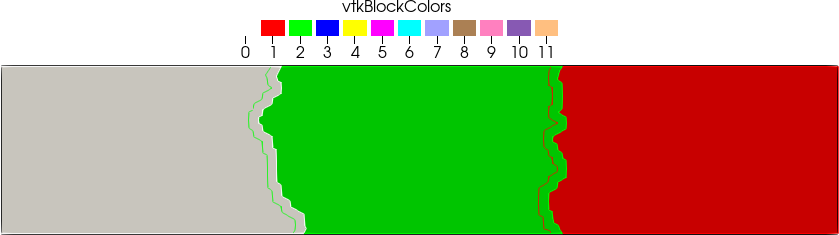
\includegraphics[align=t,width=0.4\textwidth]{./Images/le-2d-bar-partitioned3.png}\hfill
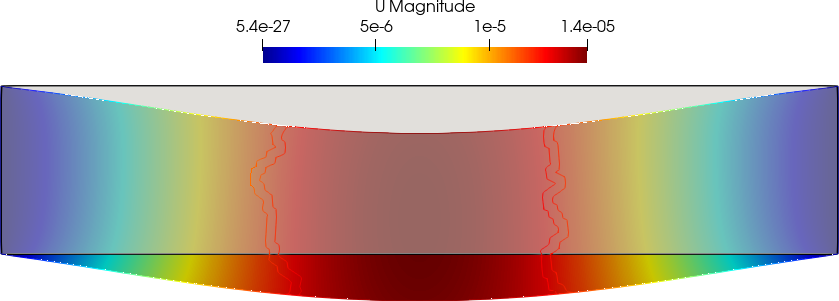
\includegraphics[align=t,width=0.4\textwidth]{./Images/le-2d-bar-clamped-ends.png}
\caption{The 2D clamped bar problem: partitioned mesh and displacement field visualization in ParaView. \label{bar-le-full-nnn}}
\end{figure}

You are all done with your 2D linear-elasticity simulation.

Try running the 3D problem. Keep in mind to rerun the
\psd{PSD\_PreProcess} with \psd{-dimension 3} flag and using the
appropriate mesh via \psd{-mesh} flag with \psd{PSD\_Solve}. It goes
without saying you will need to adjust the Dirichlet border labels in
\psd{ControlParameters.edp}.

\subsection{Redoing the test on Jupiter and Moon}

Imagine, you wish to know how the test would compare if performed on
Moon and Jupiter. Since gravity is the main force involved in the
problem, try redoing the test with different gravitational constant. The
only thing that will change now is the gravitational pull, for Moon
\(g=1.32\) and for Jupiter \(g=24.79\). To perform the moon test simply
change \psd{Fbc0Fy -10560.0} in \psd{ControlParameters.edp} and redo
step 2 and step 3. Similarly, for the Jupiter test
\psd{Fbc0Fy -198320.0} in \psd{ControlParameters.edp} and redo step 2
and step 3.

\begin{figure}[htbp]
    \centering
    \begin{minipage}[t][2.5cm][t]{0.4\textwidth}
    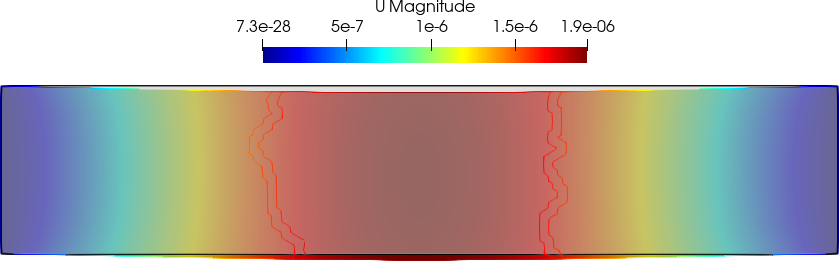
\includegraphics[align=t,width=1\textwidth]{./Images/le-2d-bar-moon.png}
    \end{minipage}\hspace{.1\textwidth}
    \begin{minipage}[t][2.5cm][t]{0.4\textwidth}
    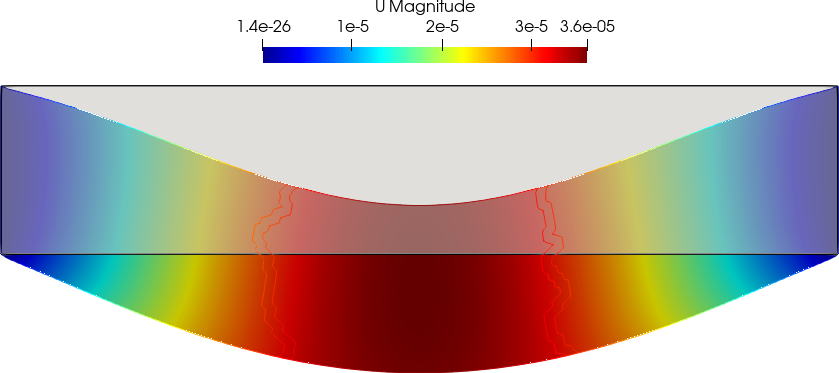
\includegraphics[align=t,width=1\textwidth]{./Images/le-2d-bar-Jupiter.png}
    \end{minipage}
    \caption{2D clamped bar 20000X warped displacement fields. On moon (left) and  on Jupiter (right).}
    \label{fig:moon-jupiter}
\end{figure}
